\title{Halt Mal Kurz}
\author{Jenny Matthiesen}
\date{\today}

\documentclass[12pt]{article}

\usepackage{booktabs}
\usepackage{textcomp}
\usepackage{array}
\usepackage{xcolor}
\usepackage{graphicx}
\graphicspath{ {./img/} }


\makeatletter
\newcommand*{\rowstyle}[1]{% sets the style of the next row
  \gdef\@rowstyle{\leavevmode#1}%
  \@rowstyle\ignorespaces}
\newcolumntype{=}{>{\gdef\@rowstyle{}}}
\newcolumntype{+}{>{\@rowstyle}}
\makeatother

\definecolor{passingzone_inv}{HTML}{CFE5A6} 
\definecolor{green_inv}{HTML}{E2A9E5} 
\setlength{\voffset}{-3cm}
\setlength{\textheight}{650pt}

\begin{document}
\maketitle

%\pagecolor{passingzone_inv}

\centering
\section*{}

\begin{tabular}{=l|+c|+c|+c|+c|+c|+c|+c|+c|+c|l}
\rowstyle{\color{gray}\scriptsize}
	& R & L & R & L & R & L & R & L & R &\\
    	Beat & 1 & 2 & 3 & 4 & 5 & 6 & 7 & 8 & 9 & \\

\toprule
	
    	A & $P_B$ & S & \colorbox{green_inv}{$P_C$} & S & \colorbox{green_inv}{$P_C$} & S & S & S & S & \textrightarrow{} C' \\
    	B & $P_A$ & S & S & S & $P_A$ & S & S & \colorbox{green_inv}{S} & - & \textrightarrow{} A' \\
	
    	C & S & S & $_PA$ & S & S & S & $P_A$ & S & S & \textrightarrow{} B' \\
\midrule
	M & $C_A$ & Zip & $S^A_C$ & - & $S^A_B$ & Zip & - & $I_B$ & - &  \textrightarrow{} M' \\
\bottomrule
\end{tabular}

\vspace{3mm}

\colorbox{green_inv}{P} To M.


\vspace{5mm}

Hands are mirrowed after every period.

\textrightarrow{} Right handed passes becomes left handed passes and vice versa. 

The mirrowed side is marked by (').

\vspace{15mm}

Walking path:

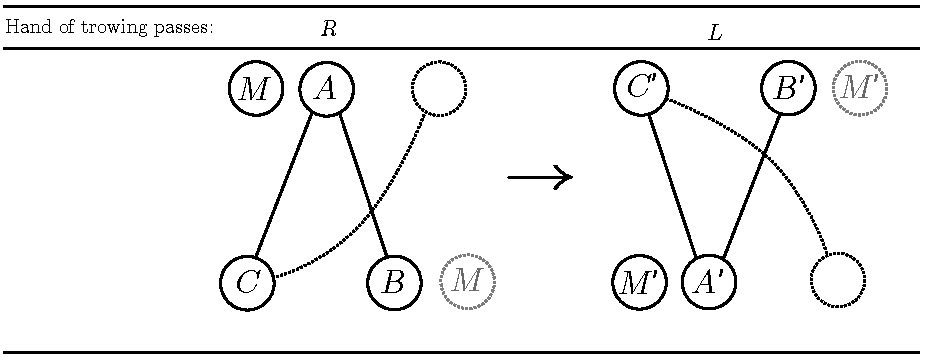
\includegraphics[width=100mm]{drawing.pdf}

\vspace{5mm}

Note that in the notation above, C is walking. The pattern can likewise be done moving to the other side, when B is walking. Then the sequence of M would be : $C_A$  $S^A_B$   $S^A_C$  $I_C$ . 

\end{document}
